%!TEX root = ../master.tex
\section{Information gatherer attacking the consumer}\label{informationGathererVsConsumer}
This section describes the attack tree for people who want to obtain private information about the consumer and use the information to construct a profile of the consumer.
Some of the possible actors that want to obtain information from the consumer are listed below:
\begin{itemize}
\item Commercial company, to better aim advertisements and commercials directly to the consumer
\item Appliance company, aiming advertisements and commercials as well as information about their market share and their competition
\item Intelligence agency, for surveillance
\item The government wanting to monitor their citizens
\end{itemize}

The attack tree can be seen on \cref{information_stealing_tree}.
The overall goal of the information gatherer is to construct a profile of the consumer.
The ``traditional'' way of doing this would be to buy this information from someone who has gathered this information.
This could be other actors from the list mentioned above, like Facebook or Google who continuously get information about its customers.
The introduction of the smart meter into the home of consumers provide a new way of collecting this information.
The sub-tree describing how to profile a customer will be described in the following sections.

\afterpage{% Insert after the current page
\cleardoublepage
\thispagestyle{plain}
\KOMAoptions{paper=A3,paper=landscape}
\recalctypearea

\begin{figure}
  \begin{center}
    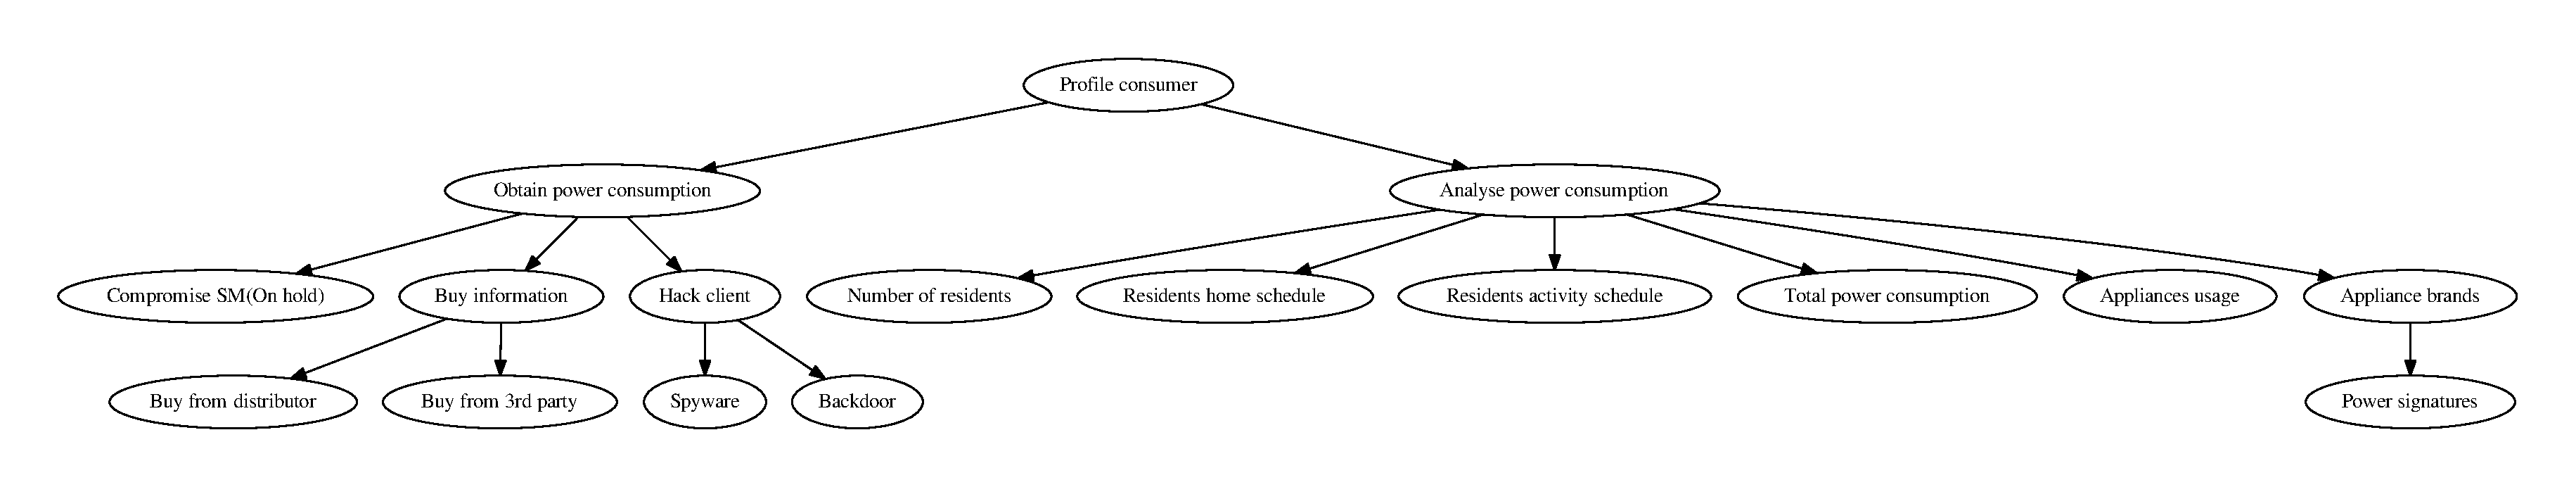
\includegraphics[width=\textwidth]{graphviz/information_stealing_vs_consumer_tree.pdf}
  \end{center}
  \caption{A information gatherer attacking the consumer by stealing his data.}
  \label{information_stealing_tree}
\end{figure}

\cleardoublepage
\KOMAoptions{paper=A4,pagesize}
\recalctypearea
}


\subsection{Obtain power consumption}
In order to analyze the consumption data of the consumer the information gatherer must obtain the consumption first.

\subsubsection{Compromise smart meter}
This subtree is similar to the subtree of the burglar getting access to the smart meter, which was discussed in \cref{compromise:SM}.
The only difference is that \emph{shoulder surfing} is omitted because the information gatherer is further away from the consumer and does not have the opportunity to get close to the consumer.

\subsubsection{Compromise client}
This subtree is similar to that of the burglar described in \cref{compromise:client}.
The only difference is the omission of the \emph{Steal client} option, again because the information gatherer is not in the immediate vicinity of the consumer.

\subsubsection{Buy power consumption}
Another possibility is to buy the information either from someone who has gained access to it or directly from the consumer.
When buying from the consumer social engineering can be used to convince the costumer to sell his data either cheap or against his will.

\subsection{Analyze power consumption}
After gaining access to the smart meter and the consumption data there are many things that can be revealed about the household and the consumers activities and appliances.
See \cref{smart_meter_privacy} to see an example of how the consumption data could be used to reveal this information.
